This section presents evaluations of the work presented in this paper. First, the compiler is evaluated. Second, the data prallelization technique is evaluated, as well as the fusion optimization, and compared to a full SkelGIS program. Third, the hybrid parallelization (data and task) is evaluated and validates the performance model detailed in Section~\ref{sect:tsp}.

All evaluations presented in this section are based on a real case study, the shallow-Water Equations. Navier-Stokes Equations is a well known set of partial differential equations in fluid dynamics to simulate a flow evolution in time. At the University of Orl\'eans, France, the MAPMO laboratory works on a software, called FullSWOF2D\footnote{\url{http://www.univ-orleans.fr/mapmo/soft/FullSWOF/}}, which solves the Shallow-Water Equations obtained from the three dimensional Navier-Stokes equations, by averaging on the vertical direction~\cite{Ferrari2004}. Those equations are solved using a two-dimensional Cartesian discretization of the space domain, and a finite volume numerical methods more described in~\cite{CPE:CPE3494}. We have developed a MSL version of FullSWOF2D that contains 3~mesh entities, 7~computation domains, 48~data and 98~computations (32~stencil kernels and 66~local kernels).

%-------------------------------------
\subsection{Compiler}

The series-parallel tree decomposition $TSP$ of this simulation, extracted by the MSL compiler, is composed of 17~sequence nodes and 18~parallel nodes. Table~\ref{fig:freq} represents the number of time a given level of parallelism, \ie the number of tasks to perform concurrently, is observed in the final tree. One can notice that the level of task parallelism extracted from the Shallow water equations is limited by two sequential parts in the application (level 1). Moreover, a level of 16~parallel tasks is reached two times, and five times for the fourth level.

\begin{table}[!h]
 \begin{center}
 \begin{tabular}{|c|c|c|c|c|c|c|c|c|}
    \hline 
   Level & 1 & 2 & 3 & 4 & 6 & 10 & 12 & 16\\
   \hline
   Frequency & 2 & 1 & 3 & 5 & 3 & 1 & 1 & 2\\
   \hline
 \end{tabular}
\caption{Parallelism level (number of parallel tasks) and the number of times this level appears.}
\label{fig:freq}
 \end{center}
\end{table}

Table~\ref{fig:exectime} illustrates the execution time for each step of the MSL compiler for an overall execution time of 4.6 seconds. Execution times have been computed on a laptop with a bi-core Intel Core i5 1.4~GHz, and 8~GB of DDR3. One can notice that the computation of the $TSP$ tree is the longest step of the compiler.

\begin{table}[!h]
 \begin{center}
 \begin{tabular}{|c|c|c|c|c|}
  \hline
   Step & Parser & $\Gamma_{sync}$ & $\Gamma_{dep}$ & $TSP$\\
   \hline
   Time (ms) & 1 & 2 & 4.2 & 3998.5\\
   \hline
   \% & 0.022 & 0.043 & 0.09 & 86.6\\
   \hline
 \end{tabular}
\caption{Execution times of the MSL compiler}
\label{fig:exectime}
 \end{center}
\end{table}

%-------------------------------------
\subsection{Data parallelism}

The first parallelization technique proposed by MSL is a data parallelization. To implement this parallelization, the dump step of the MSL compiler uses the SkelGIS language. This language, as already described, offers a distributed Cartesian mesh and programming interfaces to use it as a sequential data structure. It has been evaluated itself compared to an MPI implementation on the same FullSWOF2D simulation~\cite{}. What MSL brings to SkelGIS is an automatic detection of where MPI synchronizations are needed during the numerical simulation, and how to make a fusion of some computations in order to reduce cache misses. This section gives a performance comparison of the code produced by MSL for FullSWOF2D, and of the equivalent manual SkelGIS program (with manual synchronizations and fusion choices). Moreover, as the code produced by MSL is a component-based code, this evaluation also shows that no overheads are introduced \llc~\cite{}. Following evaluations have been performed onto the machine of the TGCC Curie described in Table~\ref{tab:TGCC}. Each evaluation has been performed ten times and the median is presented in results.

\begin{table}[!h]
\begin{center}
 \begin{tabular}{|c|c|}
   \hline
    Cluster & \textbf{TGCC Curie Thin Nodes}\\
     \hline         
    Processor & 2$\times$SandyBridge\\
    & (2.7 GHz)\\
    Cores/node & 16 \\
    RAM/node & 64 GB\\
    RAM/core & 4GB\\
    Compiler [-O3] & gcc 4.9.1\\
    MPI & Bullxmpi\\
    Network & Infiniband\\
    \hline
 \end{tabular}
 \caption{\label{tab:TGCC}Hardware configuration of TGCC Curie Thin nodes.}
 \end{center}
\end{table}

\paragraph{\textbf{Weak scaling}} The first evaluation is a weak scaling evaluation. In a weak scaling, a constant amount of work is given to each core while increasing the overall number of cores. As a result, the overall domain size also increase with the number of cores. A weak scaling is a good evaluation to detect overheads which are independent from the amount of computation performed by each core, such as collective communications, or overheads introduced by \llc components, for example. Figures~\ref{fig:weak1} and~\ref{fig:weak2} respectively show the weak scaling evaluations for a $400 \times 400$ and a $800 \times 800$ domain for each core, from 16 cores to 16.384 cores. Minimum and maximum values are also shown as error bars in figures.

\begin{figure}[!h]\begin{center}
  \resizebox{8cm}{!}{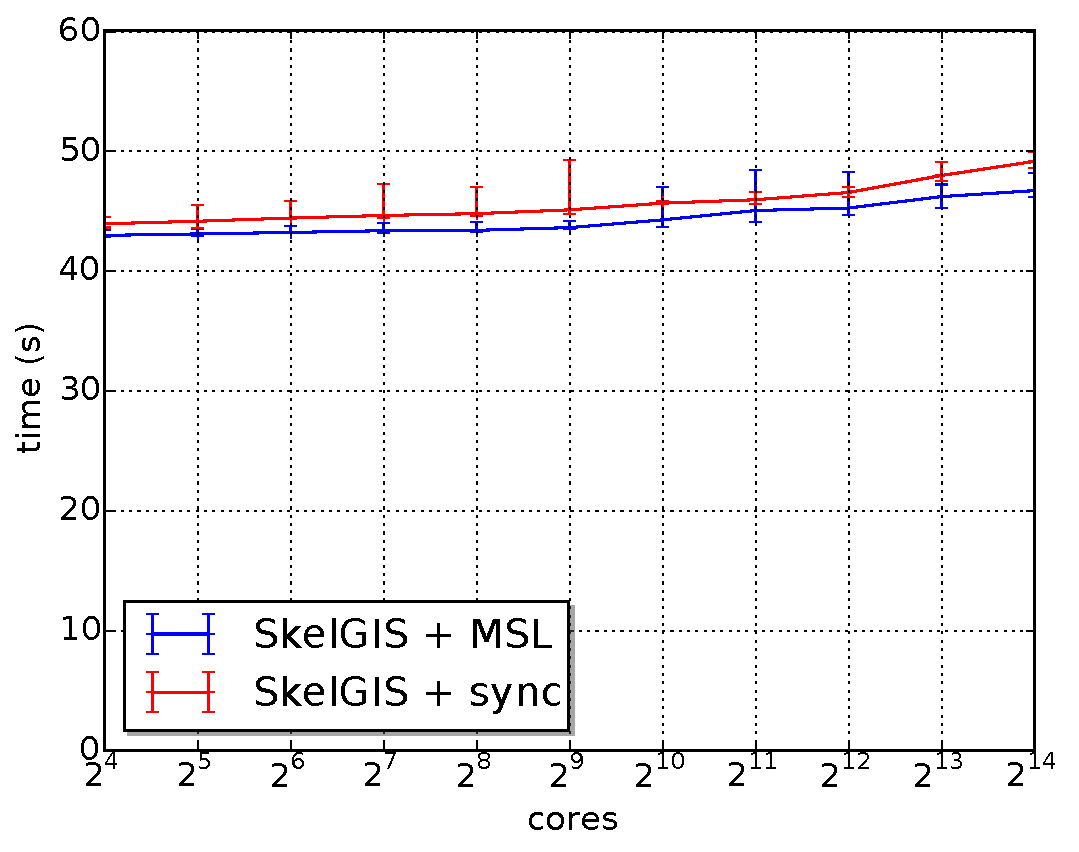
\includegraphics{../results/weak_scaling/400/median_weak.pdf}}
  \caption{weak-scaling with $400 \times 400$ domain per core.}
  \label{fig:weak1}
\end{center}\end{figure}
\begin{figure}[!h]\begin{center}
  \resizebox{8cm}{!}{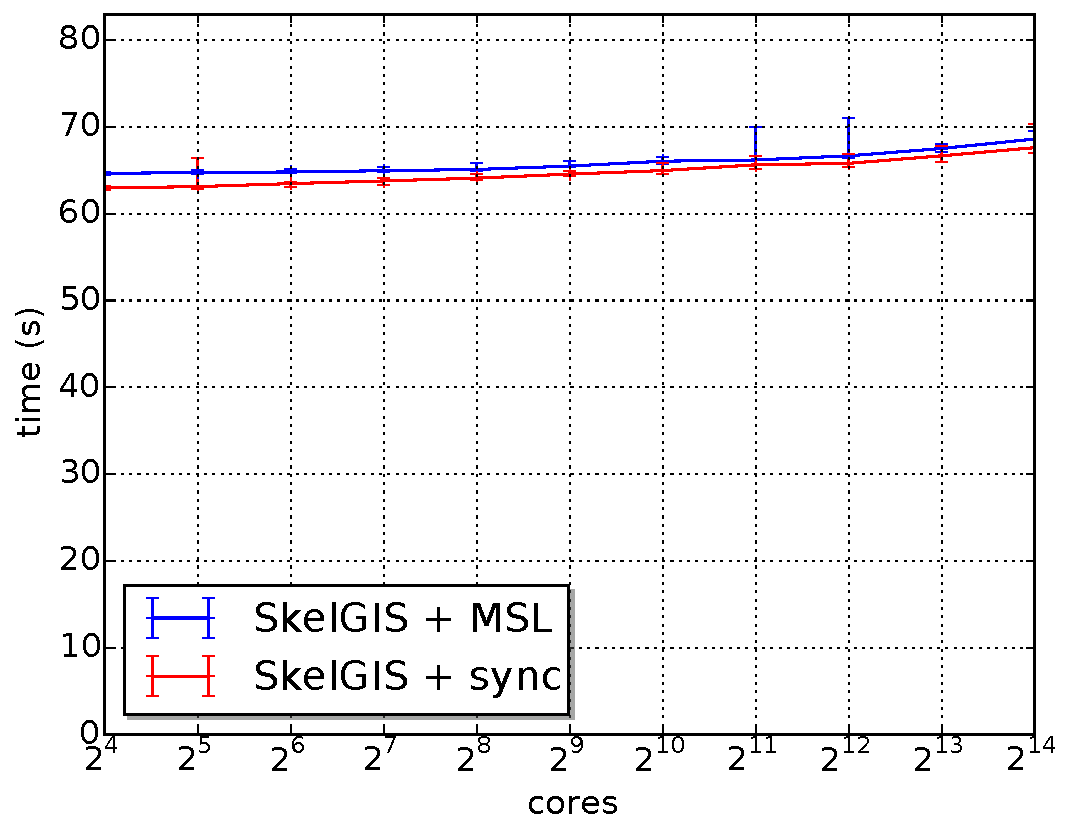
\includegraphics{../results/weak_scaling/800/median_weak.pdf}}
  \caption{weak-scaling with $800 \times 800$ domain per core.}
  \label{fig:weak2}
\end{center}\end{figure}

One can notice that the MSL code produces a better execution time on the $400 \times 400$ domain, while it produces a small overhead on the $800 \times 800$ domain. Those results could be due to different optimizations of the gcc compiler due to components. Actually, a component in \llc is compiled independently, as an dynamic library, with the \emph{-fpic} compilation option, while the SkelGIS version is compiled entirely as a single code. However, one can also notice that except those not significant differences of execution times, weak scalings have the same behavior on both codes.

\paragraph{\textbf{Strong scaling}} The second evaluation is a strong scaling evaluation. Unlike a weak scaling, a strong scaling keeps a constant overall size of problem, while the number of cores increase. As a result, the sub-domain computed by each core reduces while the number of cores increases. The strong scaling is a good additional evaluation to the weak scaling, showing different kinds of overheads, such as cache misses (when the size of sub-domain becomes small enough to fit into cache memory), or small constant overheads. Figure~\ref{fig:strong} shows the strong scaling evaluation for a $10k \times 10k$ overall domain size, from 16 cores to 16.384 cores. This strong scaling is illustrated with the number of iterations per seconds as a function of the number of cores. The ideal strong scaling is also illustrated.

\begin{figure}[!h]\begin{center}
  \resizebox{8cm}{!}{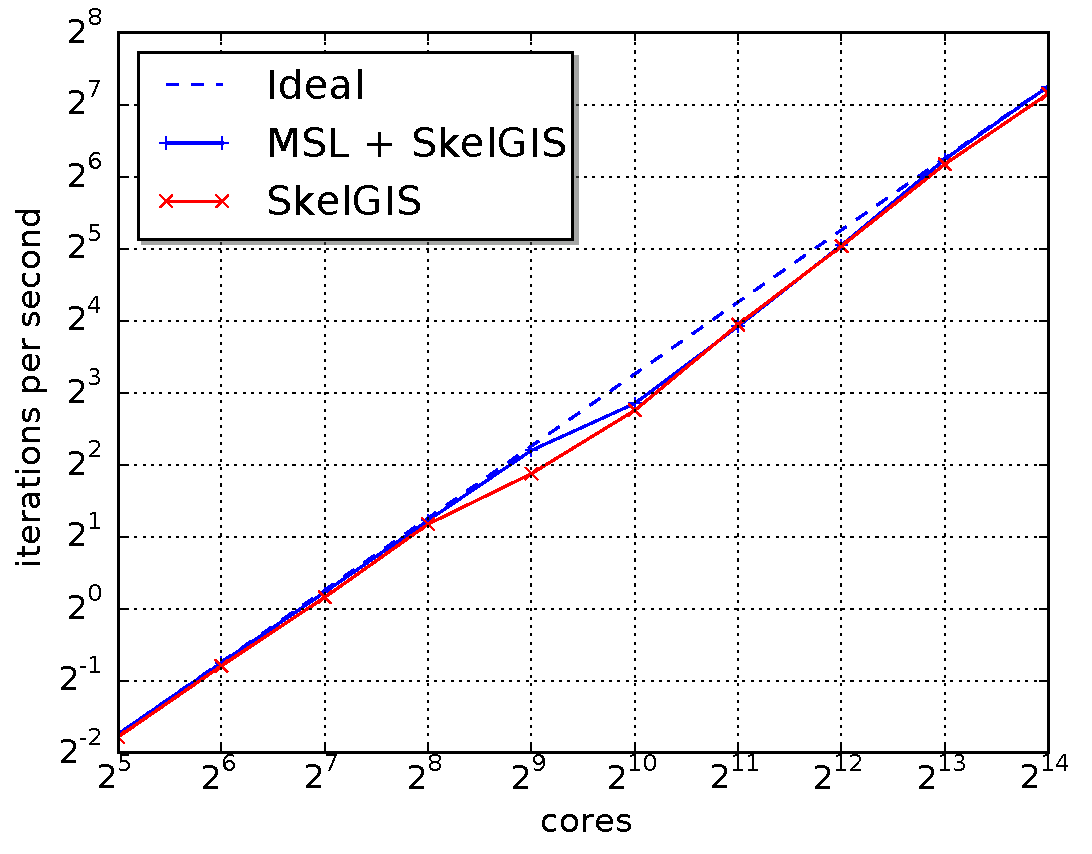
\includegraphics{../results/strong_scaling/10K_1K/median_strong.pdf}}
  \caption{Strong scaling on a $10k \times 10k$ domain.}
  \label{fig:strong}
\end{center}\end{figure}

First, one can notice that the strong scaling evaluated for the code generated by MSL is close to the ideal speedup up to 16.384 cores, which is a very good result. Moreover, no overheads are introduced by MSL which shows that automatic synchronization detections and automatic fusion detections are the same one that the one written manually into the SkelGIS code of FullSWOF2D. Finally, no overheads are introduced by components of \llc. A small behavior difference can be noticed with $2^9=512$ cores, however this variation is no longer observed with 1024 cores.

\paragraph{\textbf{Fusion}} Finally, to evaluate the data parallelization technique automatically introduced by MSL, the fusion optimization is evaluated. Figure~\ref{fig:fusion} shows the number of iterations per second as a function of the number of cores, for FullSWOF2D with and without fusion optimization and onto a $500 \time 500$ domain. As explained in Section~\ref{sect:fusion}, the MSL fusion happens at a high level and is most of the time done naturally by a computer scientist. However, for a non computer scientist which write its numerical codes, an automatic proposition of such fusions makes the implementation easier. Moreover, one can notice that the performance is clearly improved (around 40\%) by this fusion.

\begin{figure}[!h]\begin{center}
  \resizebox{8cm}{!}{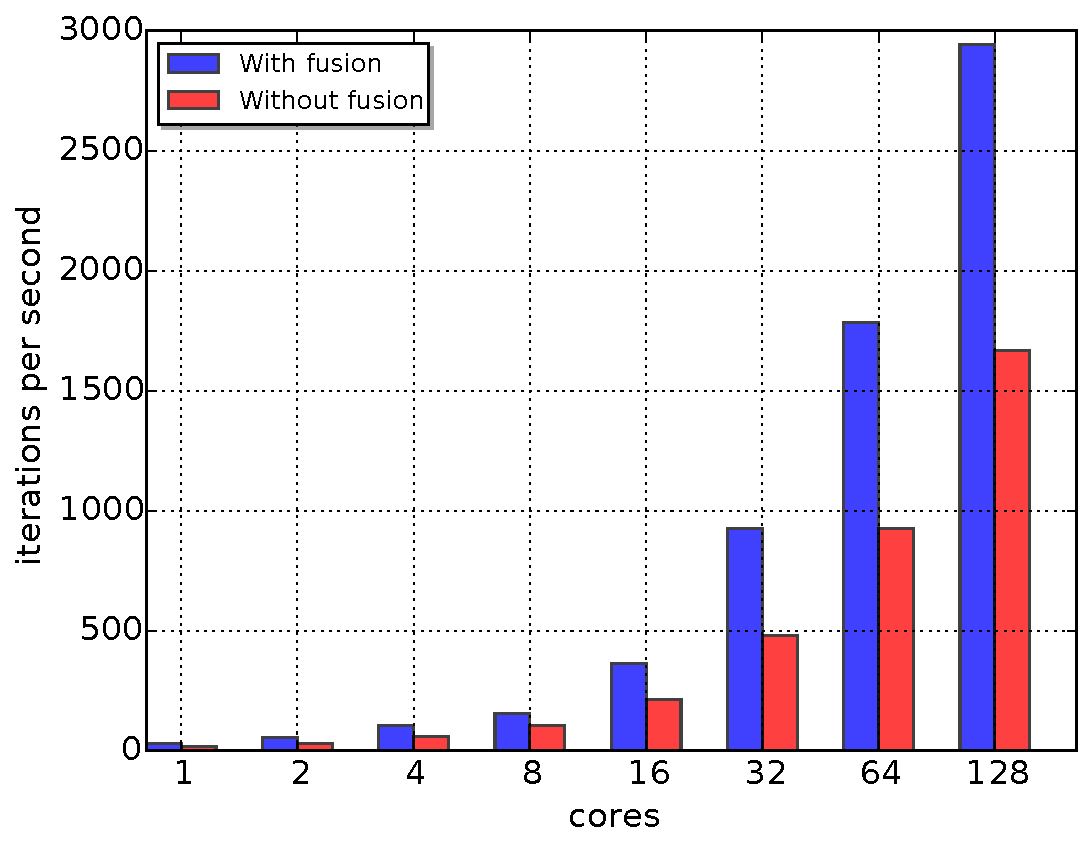
\includegraphics{../results/task_scaling/500_200/fusVSbase.pdf}}
  \caption{Strong scaling on a 500x500 domain, with and without the fusion optimization.}
  \label{fig:fusion}
\end{center}\end{figure}

%-------------------------------------
\subsection{Hybrid parallelism}

The second parallelization technique proposed by MSL is an hybrid parallelization which mixes data parallelization and task parallelization. To implement this hybrid parallelization, the dump step of the MSL compiler uses the SkelGIS language, and the OpenMP language.

First, Figure~\ref{fig:limit} illustrates limitations of data parallelization technique alone. As explained in Section~\ref{sect:perfs}, performance of data parallelism is limited by the communication time between resources. As a result, when the size of sub-domain for each core becomes too small, and as the communication time increases with the number of cores, the strong speedup of the data parallelization starts to bend down. To catch this phenomena without too much cores, a relatively small domain of $500 \times 500$ is used.

\begin{figure}[!h]\begin{center}
  \resizebox{8cm}{!}{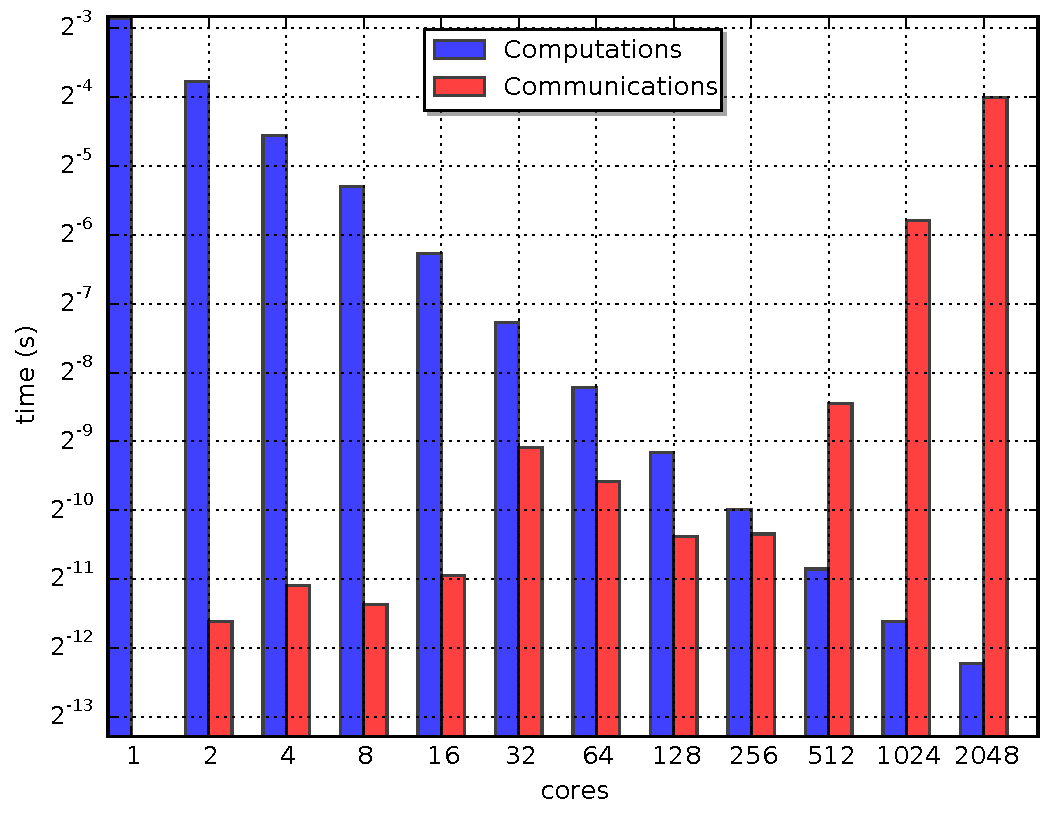
\includegraphics{../results/task_scaling/500_200/analytic/times.pdf}}
  \caption{Computation vs communication times in the data parallelization technique.}
  \label{fig:limit}
\end{center}\end{figure}

As expected, from 1 to 2048 cores the computation times decrease linearly. On the other hand, from 1 to 256 cores the communication time is almost constant, but from 256 to 2048 cores it increases. As a result from 512 cores to 2048 cores, the communication time becomes greater than the computation time. In Figure~\ref{fig:close}, the blue curve shows the strong scaling of the same example. Thus, from 256 to 2048 cores, the speedup bends down.

\medskip
In addition to the blue curve, Figure~\ref{fig:close} shows strong scalings for the same example but using an hybrid parallelization. For example, the purple curve shows the parallelization which uses 8 cores, to perform the task parallelization, for each process used for data parallelization (\ie MPI process). As a result, for example, when using 2 machines of the TGCC cluster, with a total of 32 cores, 4 cores are used for SkelGIS MPI processes, for data parallelization, and for each one 8 cores are used for task parallelization ($4 \times 8 = 32$).

As a result, and as explained in Section~\ref{sect:perfs}, data is less divided into sub-domains and the effect which is observe onto the blue curve is delayed. This figure shows a comparison with 2, 4, 8 and 16 cores per MPI process for task parallelization.

\begin{figure}[!h]\begin{center}
  \resizebox{8cm}{!}{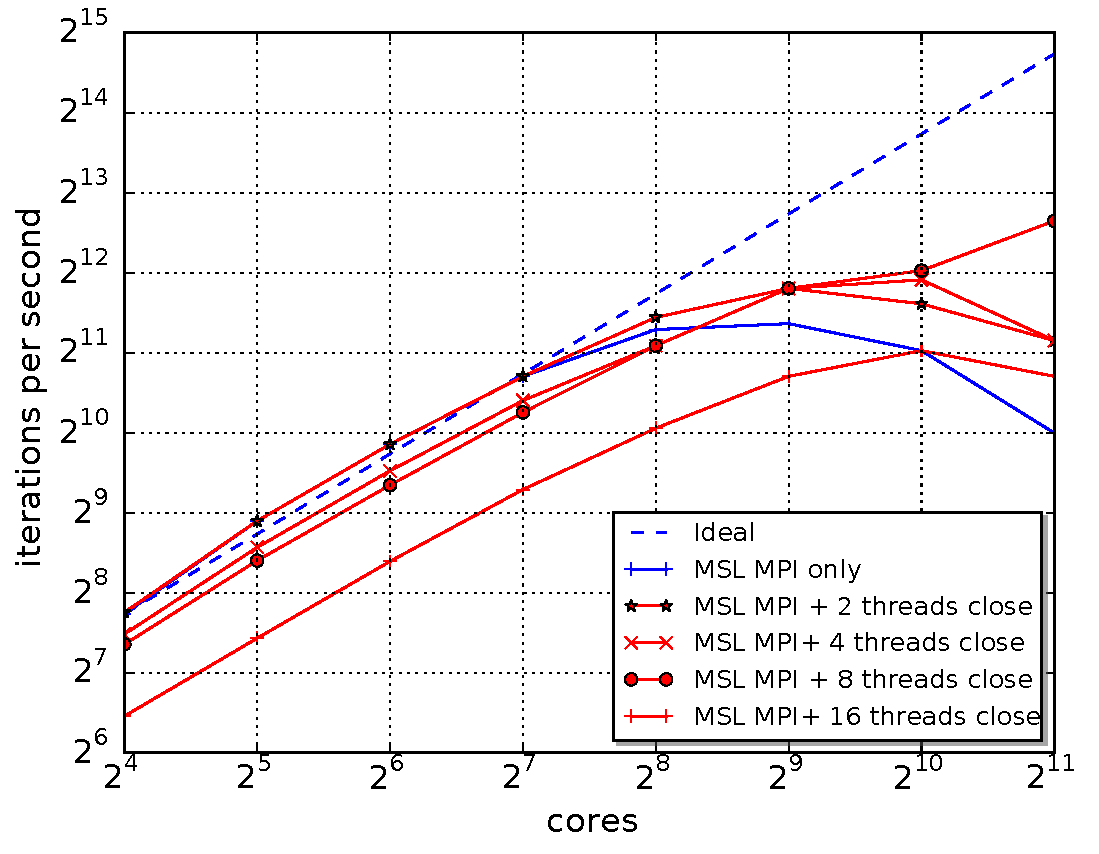
\includegraphics{../results/task_scaling/500_200/base_close_median.pdf}}
  \caption{Strong scaling comparisons between data parallelization and hybrid parallelization. A \emph{close} OpenMP clause is used to bind threads onto cores.}
  \label{fig:close}
\end{center}\end{figure}

From 2 to 8 cores, the improvement of the strong scaling is clear. However, reaching 16 cores, an important initial overhead appears and in addition to this, the curve bends down rapidly instead of improving the one with 8 cores for task parallelization. Two different phenomena happen.

First, thin nodes of the TGCC Curie are built with two NUMA nodes each of 8 cores. As a result, when increasing the number of OpenMP cores for task parallelization from 8 to 16 cores, an overhead is introduced by exchanges of data between memories of the two NUMA nodes. This phenomena is illutrated in Figure~\ref{fig:spread}. In this figure, a different strategy is used to bind threads onto available cores (using OpenMP). This strategy, called \emph{spread} instead of \emph{close} in Figure~\ref{fig:close}, binds threads on cores in order to spread as much as possible onto resources, which means that the two NUMA nodes are directly used whatever the number of cores kept for task parallelization. As a result, and as shown in the figure, using 2, 4 and 8 cores an initial overhead is introduced.

\begin{figure}[!h]\begin{center}
  \resizebox{8cm}{!}{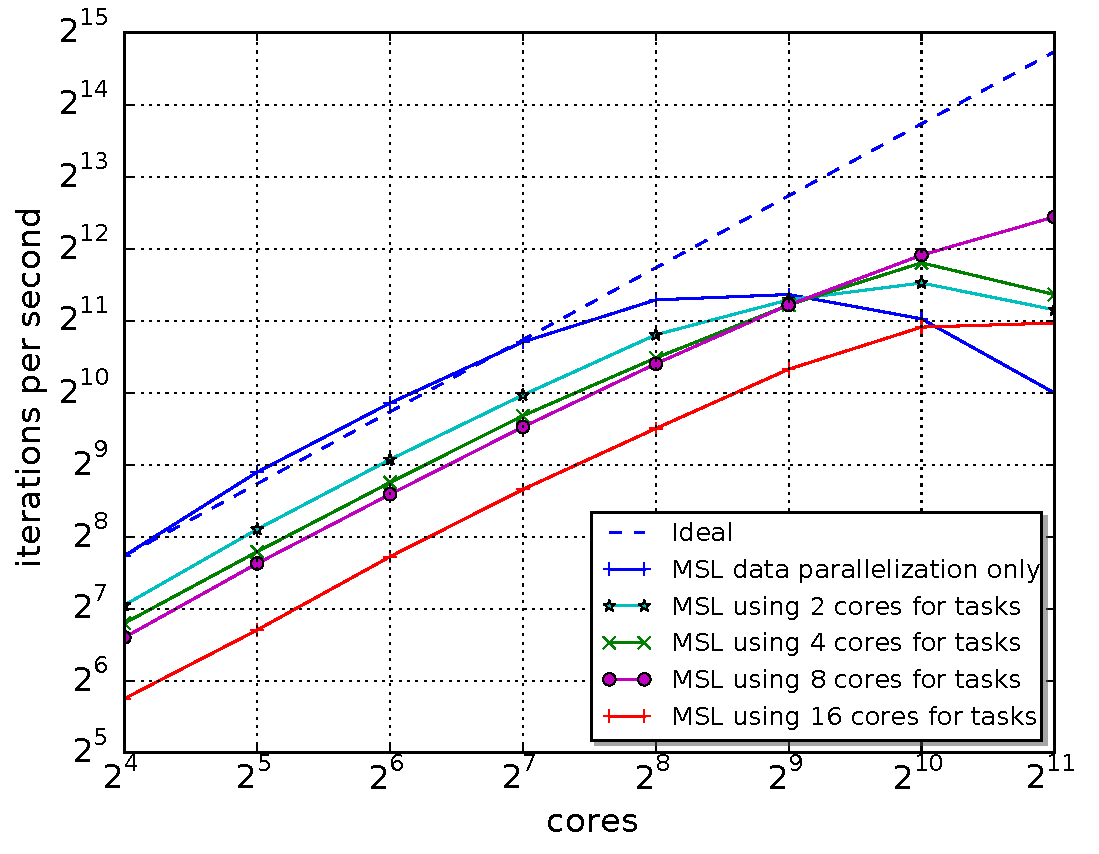
\includegraphics{../results/task_scaling/500_200/base_spread_median.pdf}}
  \caption{Strong scaling comparisons between data parallelization and hybrid parallelization. A \emph{spread} OpenMP clause is used to bind threads onto cores.}
  \label{fig:spread}
\end{center}\end{figure}

The second phenomena, which happens in Figure~\ref{fig:close} with 16 cores for tasks parallelization, is due to the level of parallelization introduced by the task parallelization technique. Actually, as illustrated in Table~\ref{fig:freq}, only two steps of the $TSP$ static scheduling generated by the MSL compiler can take advantage of 16 cores among a total of 18 steps. This phenomena has been explained in Section~\ref{sect:perfs} by the variable $F_{task}$ and the fact that it is not always true that $F_{task}=P_{task}$. This explains why using 16 cores for task parallelization in Figure~\ref{fig:spread} is still less efficient than using 8 cores even if the two NUMA nodes are always used in this evaluation.

Finally, to completely validate the performance model introduced in Section~\ref{sect:perfs}, and to understand when the hybrid parallelization becomes more interesting than the data parallelization, Figure~\ref{fig:tth2} represents $T_{COM1}$ and $T_{COM2}+T_{task}$ of Equation~(\ref{eq:hyb}), for the best case, \ie when 8 cores are used for task parallelization, and with a \emph{close} OpenMP bind of threads onto cores. Table~\ref{fig:tth} gives time details.

\begin{table}[!h]
 \begin{center}
 \begin{tabular}{|c|c|c|c|c|}
    \hline 
    & $T_{COM1}$ & $T_{COM2}$ & $T_{task}$ & Equation~(\ref{eq:hyb})\\
   \hline
   16 cores ($2 \times 8$) & 0.0005 & 0.00032 & 0.013 & False\\
   32 cores ($4 \times 8$) & 0.0018 & 0.00045 & 0.0062 & False\\
   64 cores ($8 \times 8$) & 0.0013 & 0.00038 & 0.0034 & False\\
   128 cores ($16 \times 8$) & 0.00075 & 0.0005 & 0.0023 & False\\
   256 cores ($32 \times 8$) & 0.00077 & 0.0018 & 0.001 & False\\
   512 cores ($64 \times 8$) & 0.0029 & 0.0013 & 0.00052 & True\\
   1024 cores ($128 \times 8$) & 0.018 & 0.00075 & 0.00029 & True\\
   2048 cores ($256 \times 8$) & 0.0623 & 0.00077 & 0.00016 & True\\
   \hline
 \end{tabular}
\caption{Execution times (seconds) of $T_{COM1}$, $T_{COM2}$ and $T_{task}$ for 8 cores for task parallelization. Verification of the Equation~(\ref{eq:hyb}).}
\label{fig:tth}
 \end{center}
\end{table}

\begin{figure}[!h]\begin{center}
  \resizebox{8cm}{!}{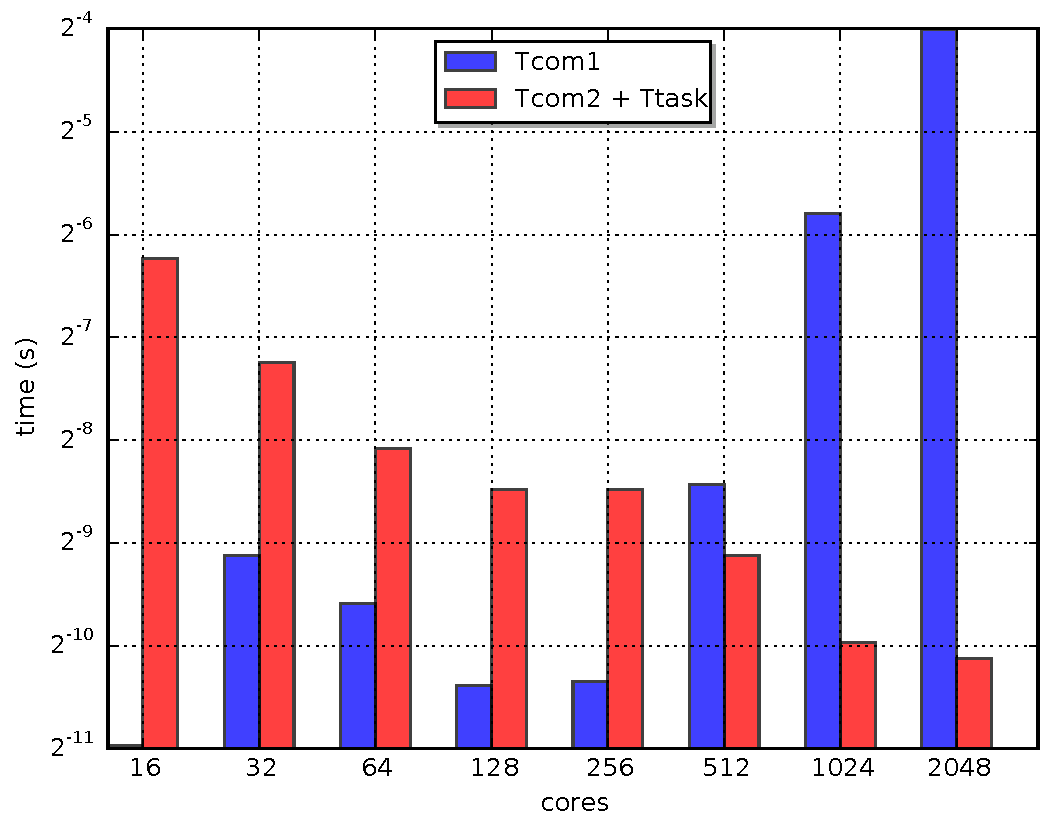
\includegraphics{../results/task_scaling/500_200/analytic/tth.pdf}}
  \caption{Execution times (seconds) of $T_{COM1}$ and $T_{COM2} + T_{task}$ for 8 cores for task parallelization. Verification of the Equation~(\ref{eq:hyb}).}
  \label{fig:tth2}
\end{center}\end{figure}

Figure~\ref{fig:tth2} and Table~\ref{fig:tth} perfectly matches results observed in Figure~\ref{fig:close} for 8 cores used for task parallelization per core used for data parallelization. As a result, the hybrid parallelization becomes better with a total of 512 cores.
